% ------------------------------------------------
% Page start
% ------------------------------------------------
\chapter{Performance Evaluation}
\label{chapter:performance-evaluation}

\baselineskip=26pt
\thispagestyle{empty}
% ------------------------------------------------

% Time evaluation section
\subsection{Time evaluation}

% Setup section
\subsubsection{Setup}

To measure the performance of Li's Hash by measuring the time of each data type (except BLOB) and operation and compare with SQLite \cite{web:sqlite:home-page}, MariaDB \cite{web:mariadb:home-page} and PostgreSQL \cite{web:postgresql:home-page} by using single table in memory to remove any possible I/O delay.\\

There is no SQL parser for Li's Hash which may this test un-fair, but a SQL parser can't too slow because it is one of core part for a SQL database. We observe the timing of SQLite and it take < 0.001 ms per SQL on our platform. So it seem that the time is too small that can be ignore.\\

Also, because normally the real hash table will use the index as a pointer, but the problem is that kind of hash table need to use a static array, but a dynamic hash table that even the std::map in standard C++ library, it still need to use the $\log(n)$ like the other B+ tree does.\\

So if still use these kind library as our back-end storage to do the testing which will not see the improvement of our design, so that we implemented our own back-end storage based on Radix tree \cite{web:wiki:radix-tree} and it work similar as the design of the Linux kernel does \cite{web:linux-kernel:radix-tree}.\\

%\begin{figure}[h]
%\centering
%\includegraphics[scale=0.5]{./performance/pic/a.png}
%\caption{The Radix tree design.}
%\label{fig:performance:}
%\end{figure}

%Figure \cite{fig:performance:} is our design look like, we hash the key become a number (Same as the ring design in Dynamo \cite{paper:amazon-dynamo-1}), next convert the number into byte array which that the index will become its' depth and the value of the byte will be as its' index number for moving to the downward, until found the leaf which is the data storage.\\

%Collision is very easy happen in hash function, we can do two way to slove it in our tree design:

%\begin{enumerate}

%\item \textbf{Increase the depth of tree}\\
%Increase the byte length of the hash function output, which means incease the depth of tree.

%\item \textbf{Multi-level tree}\\
%Our Radix tree can become a multi-level tree, will mean the leaf can become the root of the next level tree.

%The reason of this design is a single hash function still can cause a very small collision, so if using a tree that build from multi-hash function that should highly decrease the collision probelm.

%\end{enumerate}

% Testing section
\subsection{Testing}

We use the default configure for SQLite base on assume the user is new for it, then he/she will only care the performance in the default, also the default is set by the offical that what they think is the best, so this can be as a baseline of the database.\\

%We use 100,000 rows (keys) for test the performance on our platform. The reason is because we tested up to 500,000 and found out when SQLite enabled the indexing, the average time per SQL seem very static, so testing more rows seem don't prodive any useful information.

% Hardware table

\begin{table}[ht]
\centering
\label{table:performance:testing-platform}
\begin{tabular}{|c|c|}

\hline
\multicolumn{1}{|r|}{CPU:} &
\multicolumn{1}{c|}{Intel Xeon E5-2620} \\

\hline
\multicolumn{1}{|r|}{RAM:} &
\multicolumn{1}{c|}{180 GB} \\

\hline
\multicolumn{1}{|r|}{OS:} &
\multicolumn{1}{c|}{Ubuntu 12.04.4} \\

\hline
\multicolumn{1}{|r|}{Kernel:} &
\multicolumn{1}{c|}{3.11.0-15-generic} \\

\hline
\multicolumn{1}{|r|}{GCC version:} &
\multicolumn{1}{c|}{4.6.3} \\

\hline
\multicolumn{1}{|r|}{SQLite version:} &
\multicolumn{1}{c|}{3.8.1} \\

\hline
\end{tabular}
\end{table}



\clearpage

% ----------------------------------------------------------

\begin{enumerate}


%In this layer, we test the baseline of all databases without using the index, but without index the Li's Hash can't do query as a normal non-relational database. So we only test the performance of the back-end database by only use the basic put(), get() for all data type in Li's Hash. Also only use normal SELECT, INSERT in relational database without enable index.\\

% Database layer section
\item \textbf{Database layer}

In this layer, we test the baseline of both databases without using the index, but without index the Li's Hash can't do query as a normal non-relational data-base. So we only test the performance of the back-end data-base by using the basic \textit{put()}, \textit{get()} for all data type in Li's Hash. Also only use normal SELECT, INSERT in relational database without enable index. We use the code in table \ref{table:performance:database-layer:code-example} to do this test.\\

% Database layer test table 

% Database layer test
\begin{table*}
\centering
\caption{Example code that to test STRING type in \textit{Database layer}}
\label{table:performance:database-layer:code-example}
\begin{tabular}{|c|c|c|}

\hline
\multicolumn{1}{|c|}{} &
\multicolumn{1}{c|}{\textbf{Li's Hash}} &
\multicolumn{1}{c|}{\textbf{Relational database}} \\

\hline
\multicolumn{1}{|c|}{Create table} &
\multicolumn{1}{c|}
{\tabincell{c}{
X \\ (Key-value store don't need table)
}} &
\multicolumn{1}{l|}{CREATE TABLE table(value TEXT) ;} \\

\hline
\multicolumn{1}{|c|}{Insert} &
\multicolumn{1}{l|}{put('key-\textit{i}', 'value-\textit{i}')} &
\multicolumn{1}{l|}{INSERT INTO table('value') VALUES ('value-\textit{i}') ;} \\

\hline
\multicolumn{1}{|c|}{Select} &
\multicolumn{1}{l|}{get('key-\textit{i}')} &
\multicolumn{1}{l|}{SELECT value FROM table LIMIT \textit{i}, 1 ;} \\

\hline
\end{tabular}
\end{table*}



% Database layer result

\begin{figure*}
\centering
%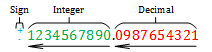
\includegraphics[scale=1.0]{./algorithm/real/pic/design/data_format_v2.png}
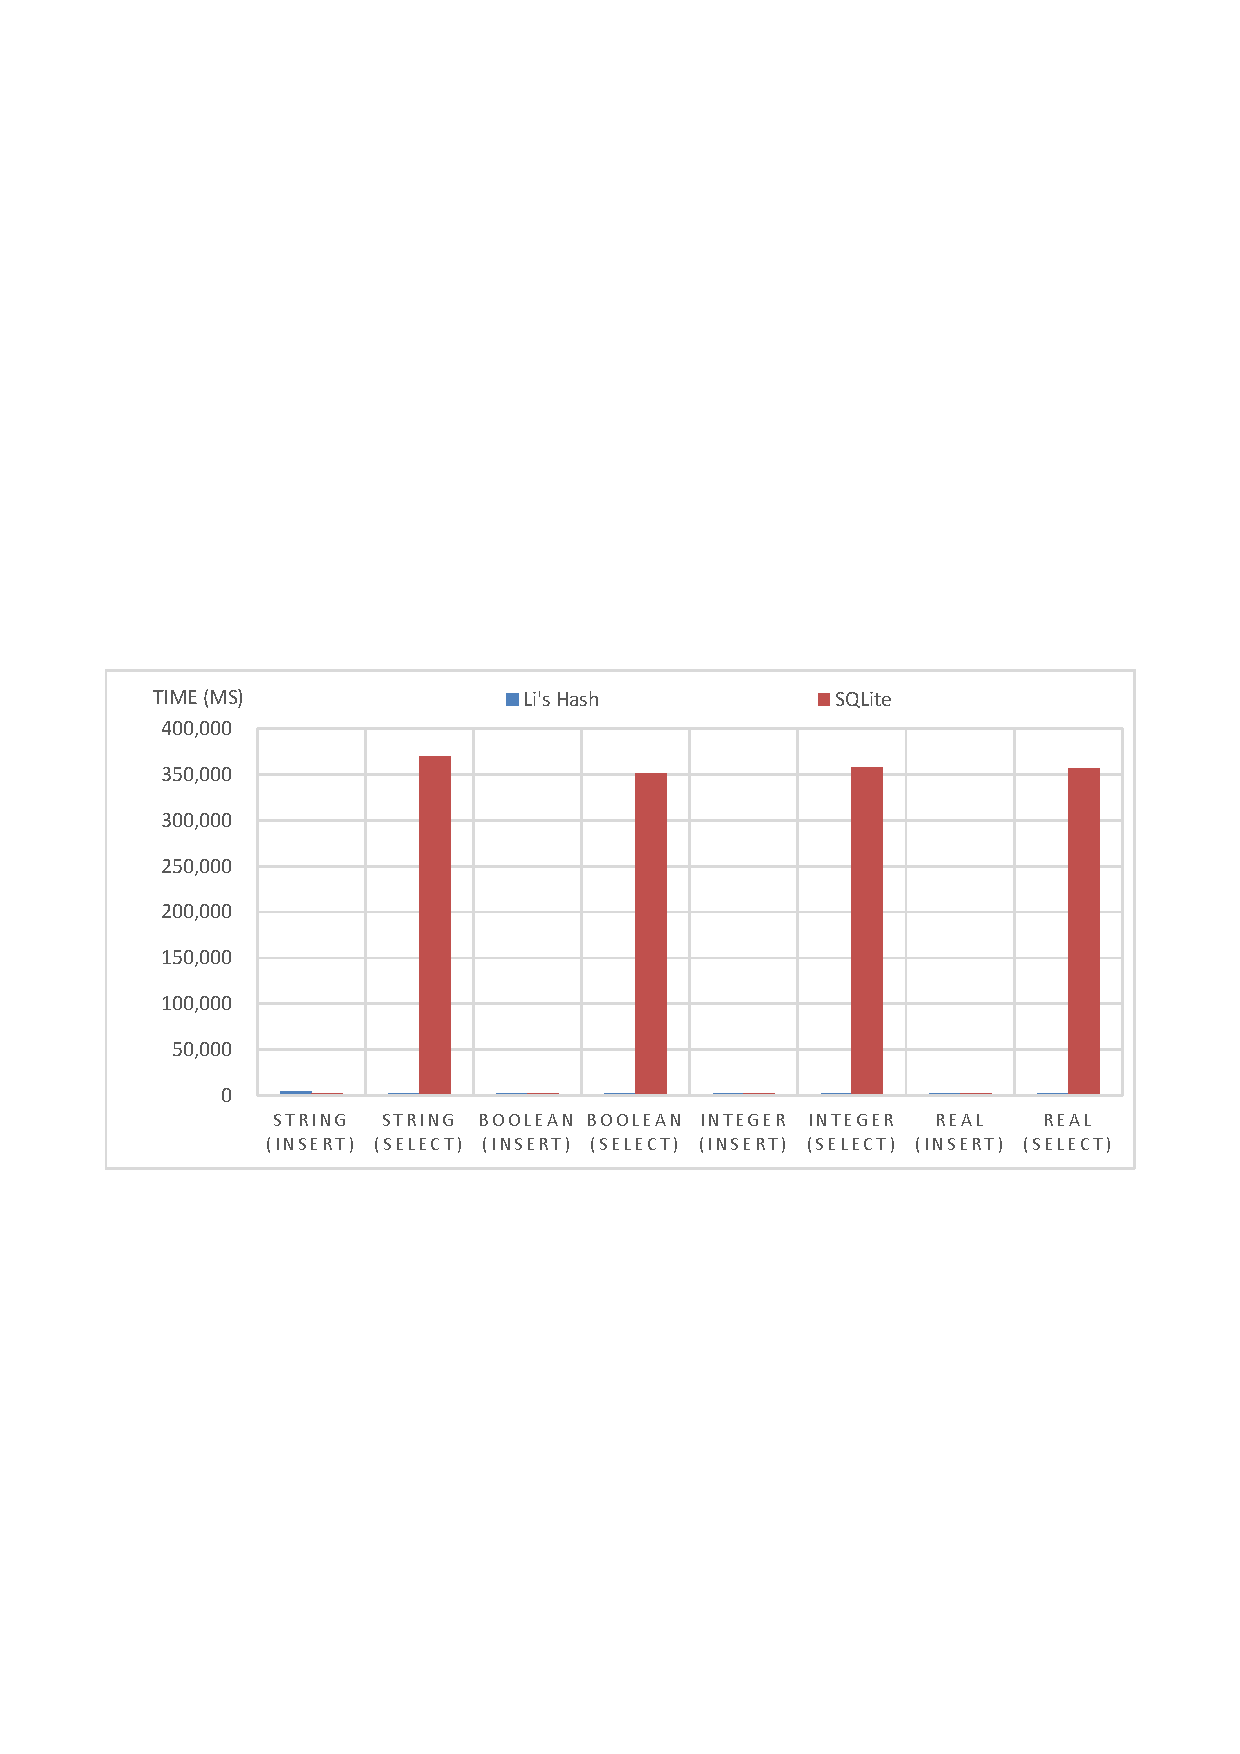
\includegraphics[width=0.8\textwidth]{./performance/result/database-layer/image/100only/full2.pdf}
\caption{Performance on database layer}
\label{fig:performance:result:database-layer}
\end{figure*}



\clearpage

% ----------------------------------------------------------

% Index layer section
\item \textbf{Index layer}

Fellow the test in \textit{Database layer}, but this time we include the index part, remove(), update() for Li's Hash. Also test DELETE, UPDATE with enable the index in relational database which using the code of table \ref{table:performance:index-layer:code-example}.\\

% Index layer test table 

% Index layer test
\begin{table*}[width=\textwidth]
\centering
\caption{Example code that to test STRING type in \textit{Index layer}}
\label{table:performance:index-layer:code-example}
\begin{tabular}{|c|c|c|}

\hline
\multicolumn{1}{|c|}{} &
\multicolumn{1}{c|}{\textbf{Li's Hash}} &
\multicolumn{1}{c|}{\textbf{Relational database}} \\

\hline
\multicolumn{1}{|c|}{Create table} &
\multicolumn{1}{l|}
{\tabincell{l}{
create\_table('table', 'value', STRING\_TYPE)
}} &
\multicolumn{1}{l|}
{\tabincell{l}{
CREATE TABLE table(id INT, value TEXT) ; \\
CREATE INDEX idx\_value ON table (value) ;
}} \\

\hline
\multicolumn{1}{|c|}{Insert} &
\multicolumn{1}{l|}
{\tabincell{l}{
insert('table', 'value-\textit{i}')
}} &
\multicolumn{1}{l|}
{\tabincell{l}{
INSERT INTO table('value') VALUES ('value-\textit{i}') ;
}} \\

\hline
\multicolumn{1}{|c|}{Select} &
\multicolumn{1}{l|}
{\tabincell{l}{
select('table', 'value', 'value-\textit{i}')
}} &
\multicolumn{1}{l|}
{\tabincell{l}{
SELECT value FROM table \\
WHERE value = 'value-\textit{i}' ;
}} \\

\hline
\multicolumn{1}{|c|}{Update} &
\multicolumn{1}{l|}
{\tabincell{l}{
update('table', 'value', 'value-\textit{i}', 'value-\textit{i}-')
}} &
\multicolumn{1}{l|}
{\tabincell{l}{
UPDATE table SET 'value' = 'value-\textit{i}-' \\
WHERE value = 'value-\textit{i}' ;
}} \\

\hline
\multicolumn{1}{|c|}{Remove} &
\multicolumn{1}{l|}
{\tabincell{l}{
remove('table', 'value', 'value-\textit{i}-')
}} &
\multicolumn{1}{l|}
{\tabincell{l}{
DELETE FROM table WHERE value = 'value-\textit{i}' ;
}} \\

\hline
\end{tabular}
\end{table*}



% Index layer result 

\begin{figure*}
        \centering

        \begin{subfigure}[b]{0.4\textwidth}
                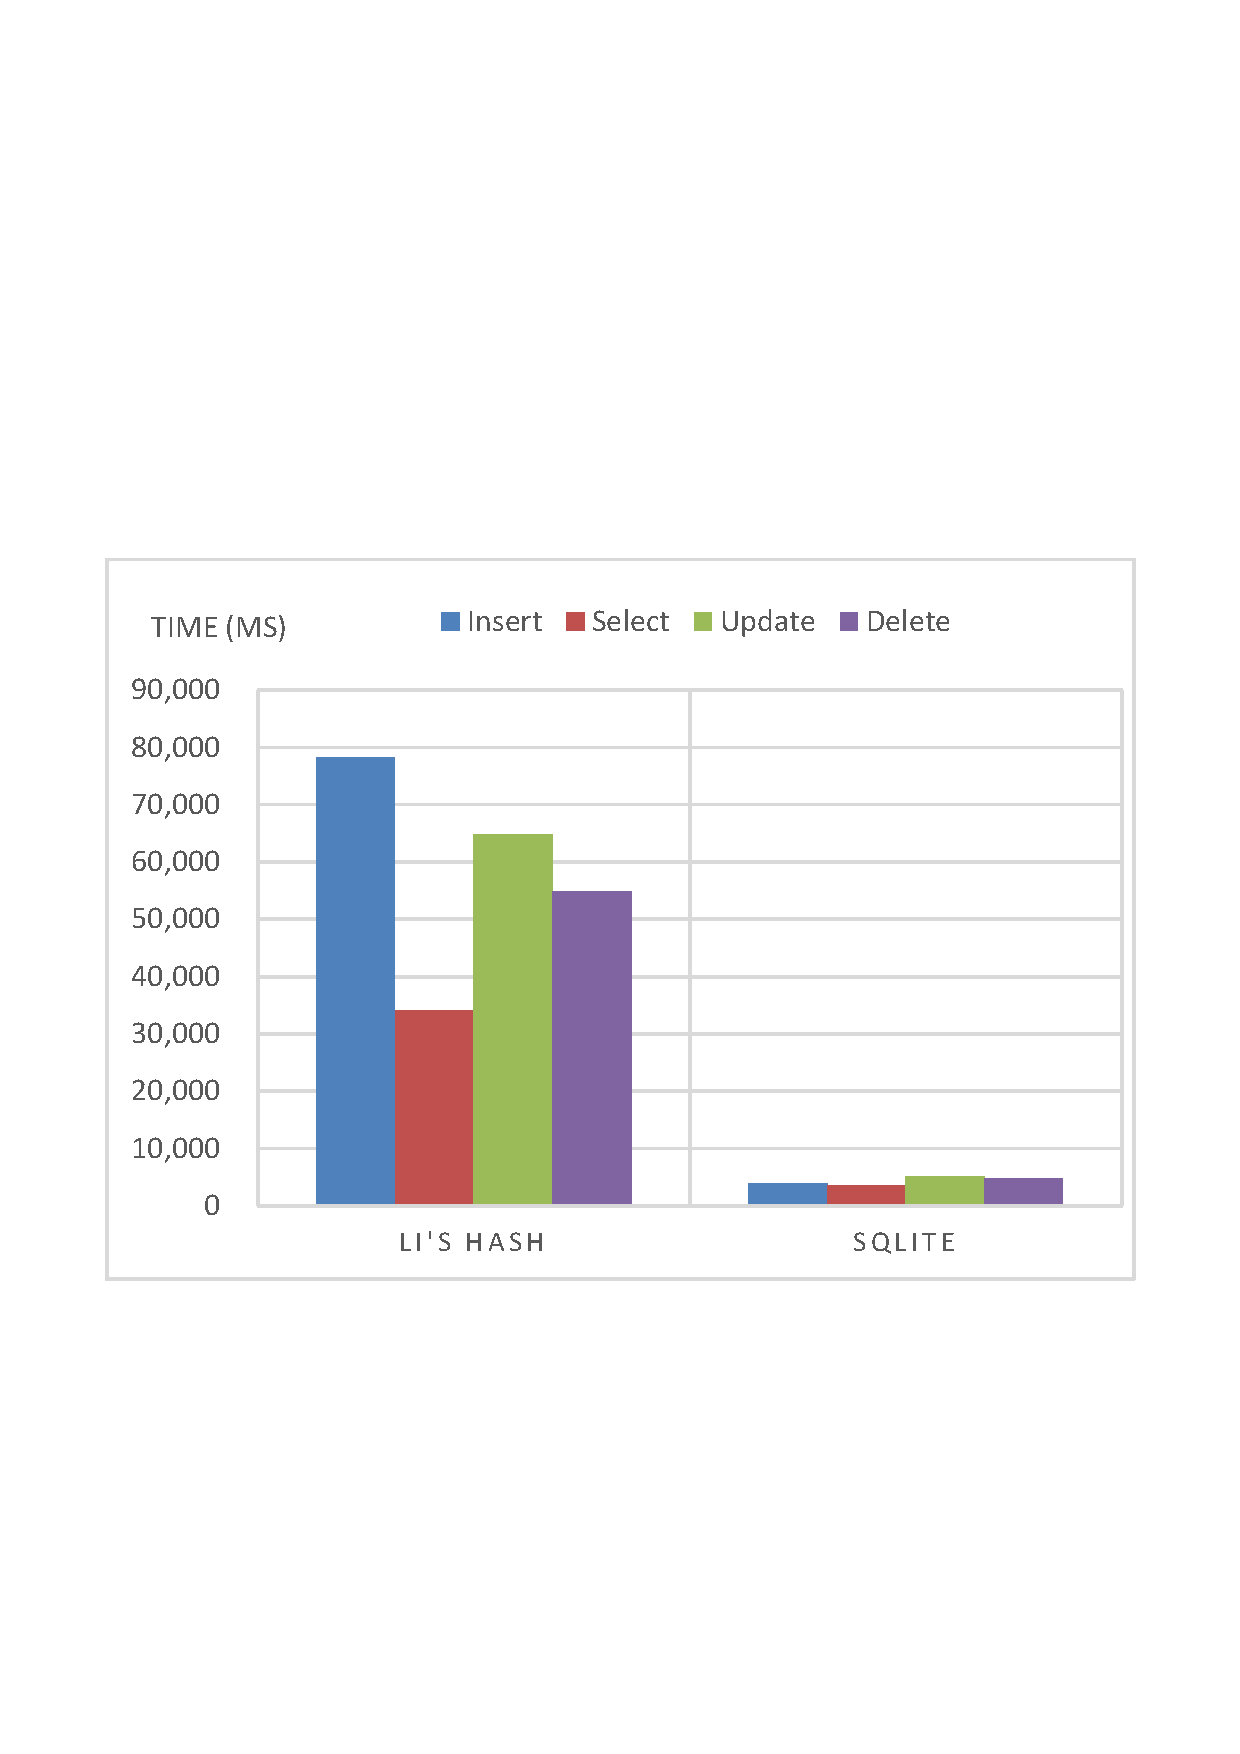
\includegraphics[width=\textwidth]{./performance/result/index-layer/image/100only/string1.pdf}
                \caption{STRING type}
                \label{fig:performance:result:index-layer:insert:boolean}
        \end{subfigure}%
        ~ %add desired spacing between images, e. g. ~, \quad, \qquad etc.
          %(or a blank line to force the subfigure onto a new line)
        \begin{subfigure}[b]{0.4\textwidth}
                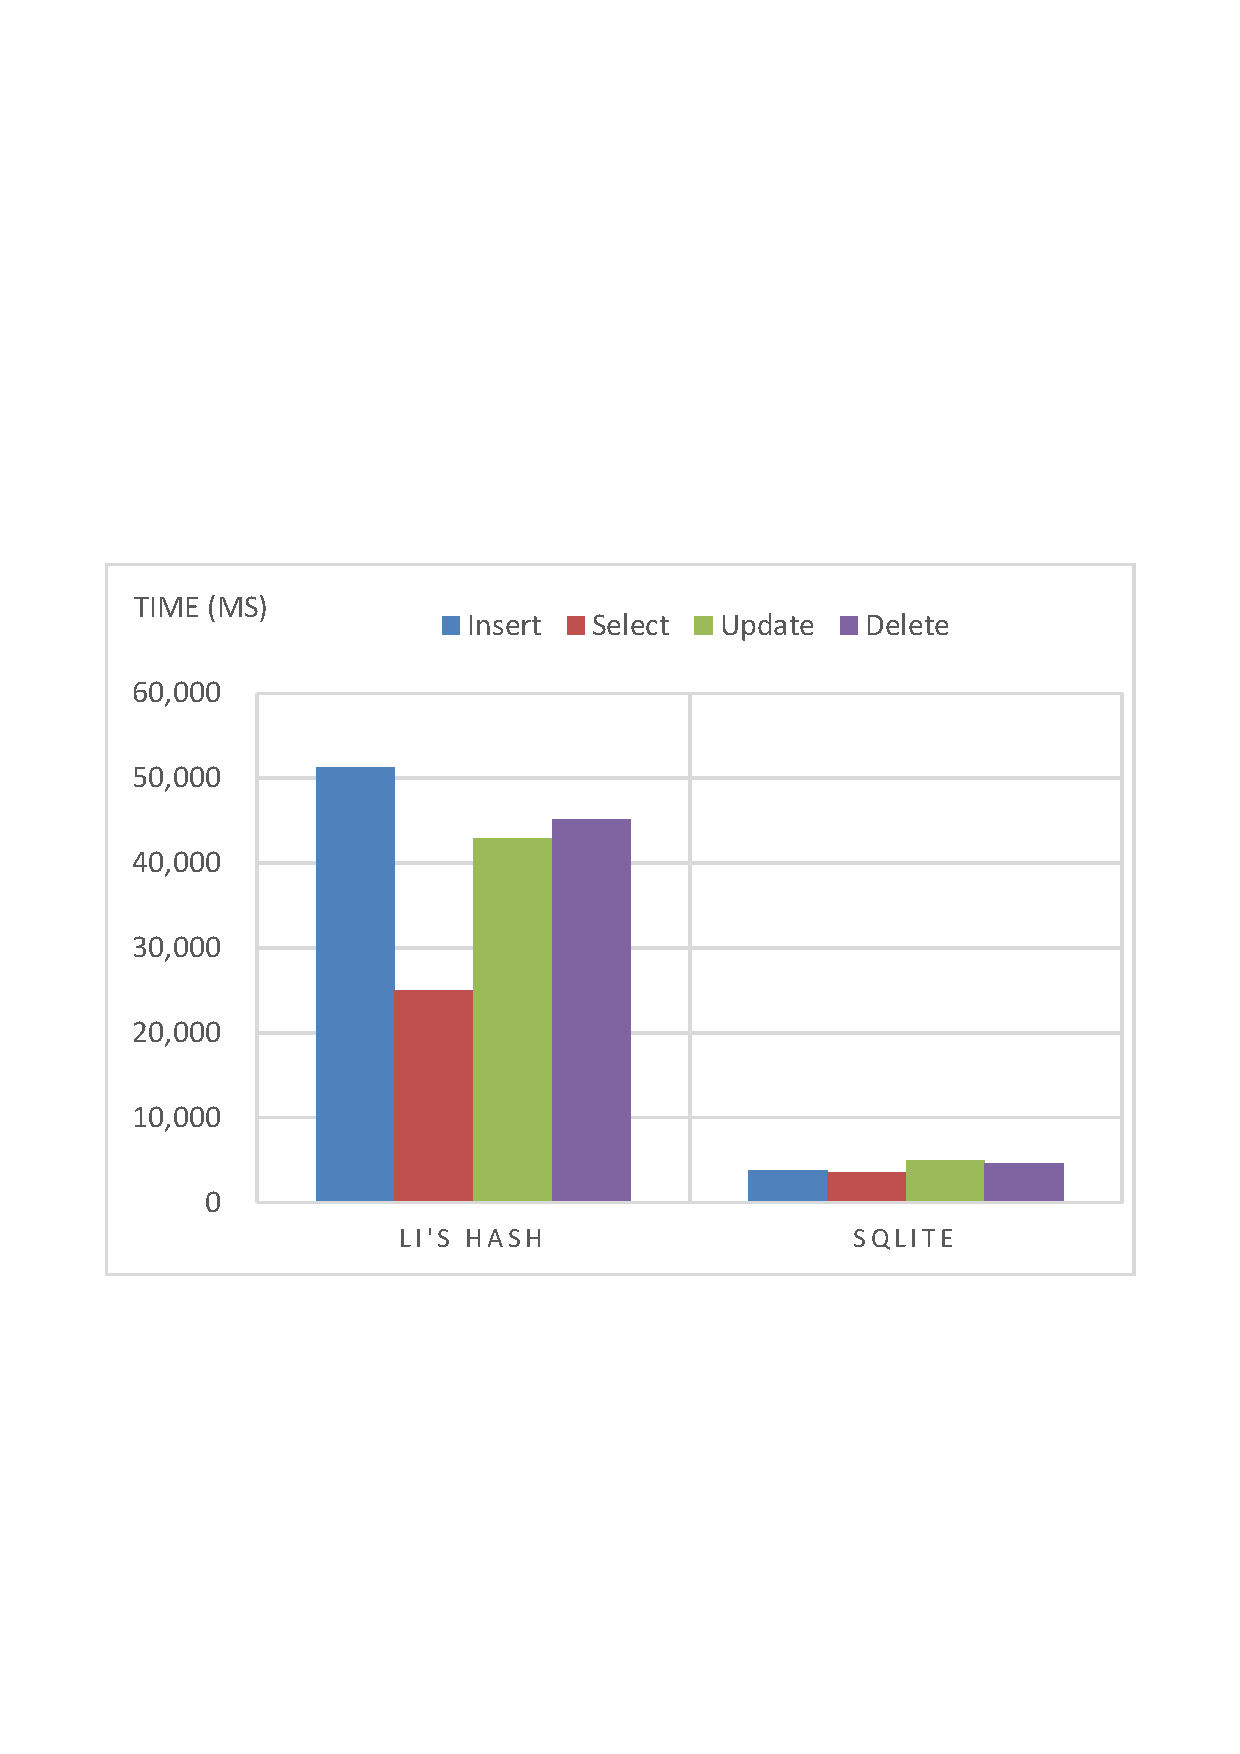
\includegraphics[width=\textwidth]{./performance/result/index-layer/image/100only/boolean1.pdf}
                \caption{BOOLEAN type}
                \label{fig:performance:result:index-layer:insert:int}
        \end{subfigure}

        \begin{subfigure}[b]{0.4\textwidth}
                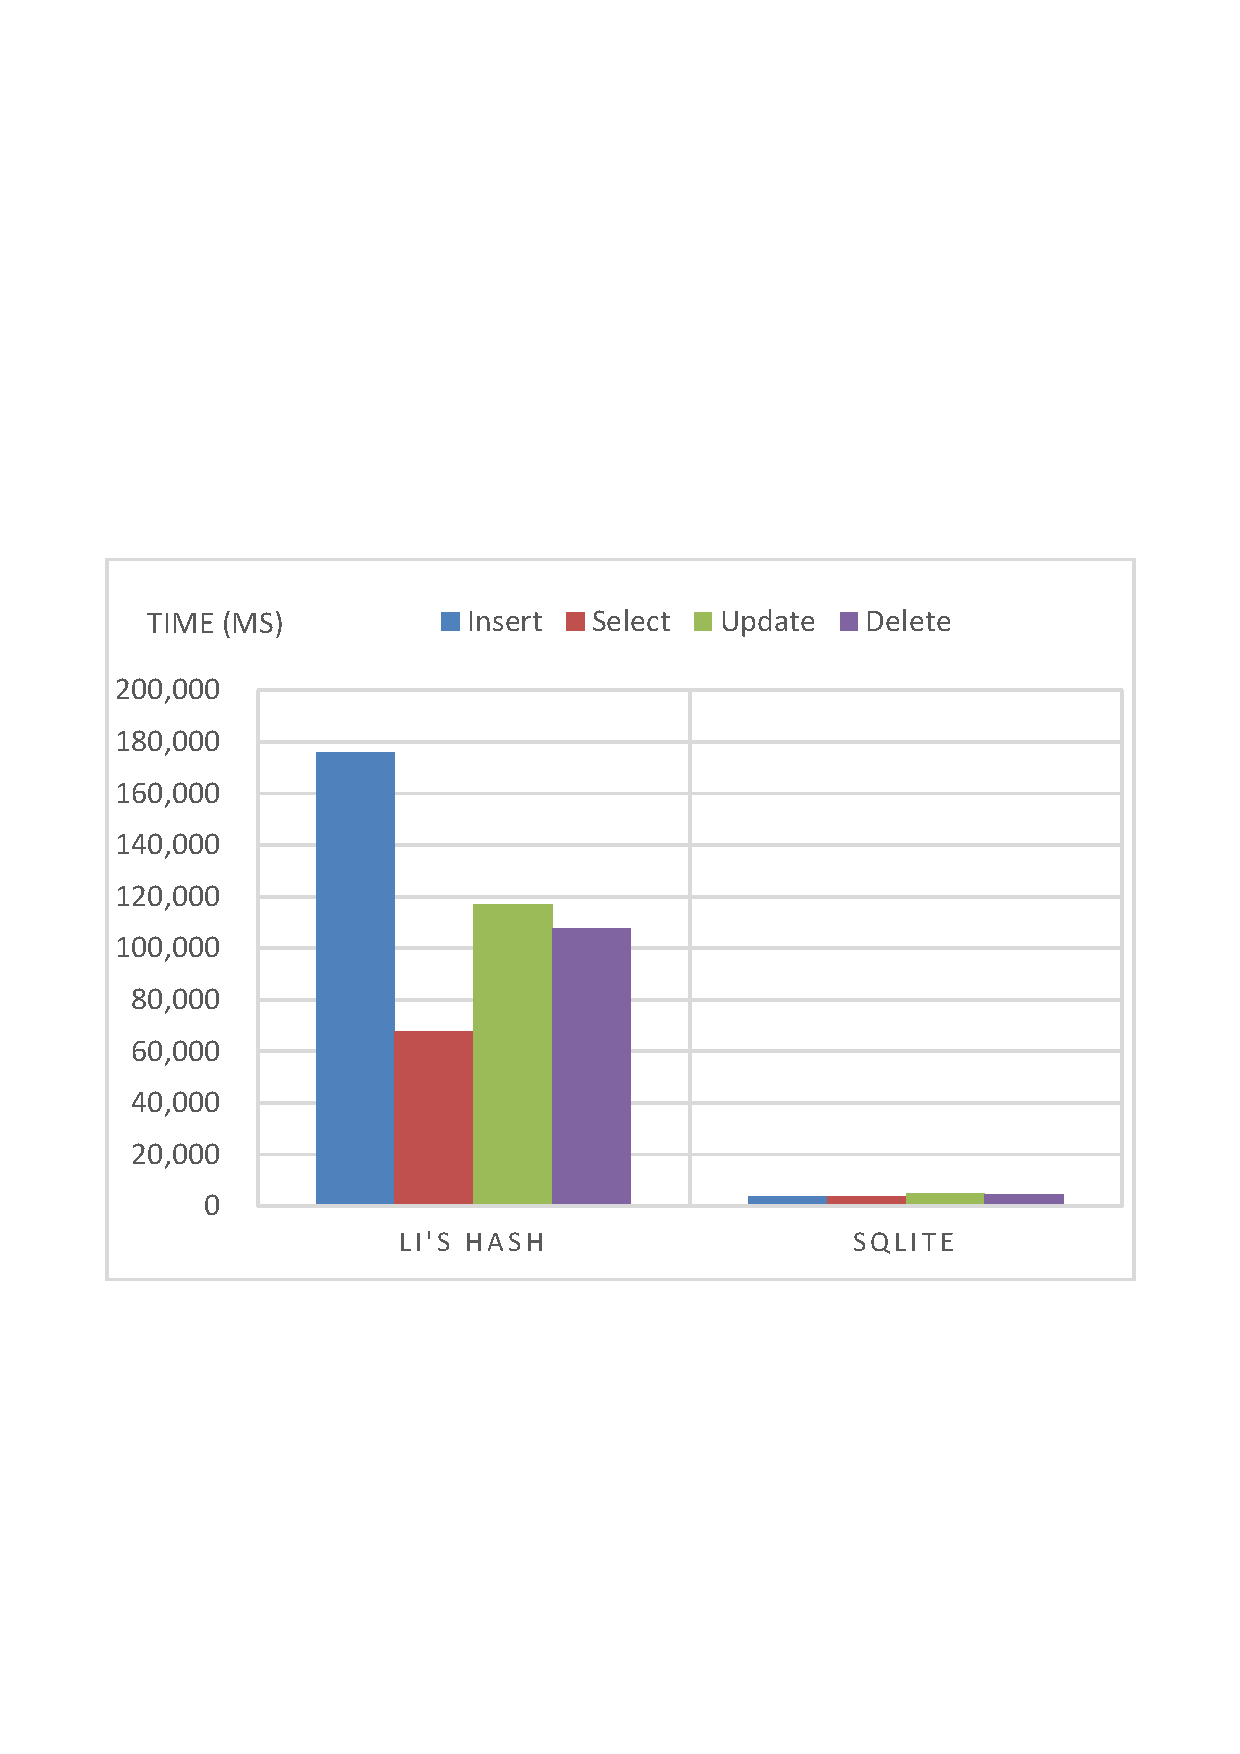
\includegraphics[width=\textwidth]{./performance/result/index-layer/image/100only/integer1.pdf}
                \caption{INTEGER type}
                \label{fig:performance:result:index-layer:insert:real}
        \end{subfigure}
        ~ %add desired spacing between images, e. g. ~, \quad, \qquad etc.
          %(or a blank line to force the subfigure onto a new line)
        \begin{subfigure}[b]{0.4\textwidth}
                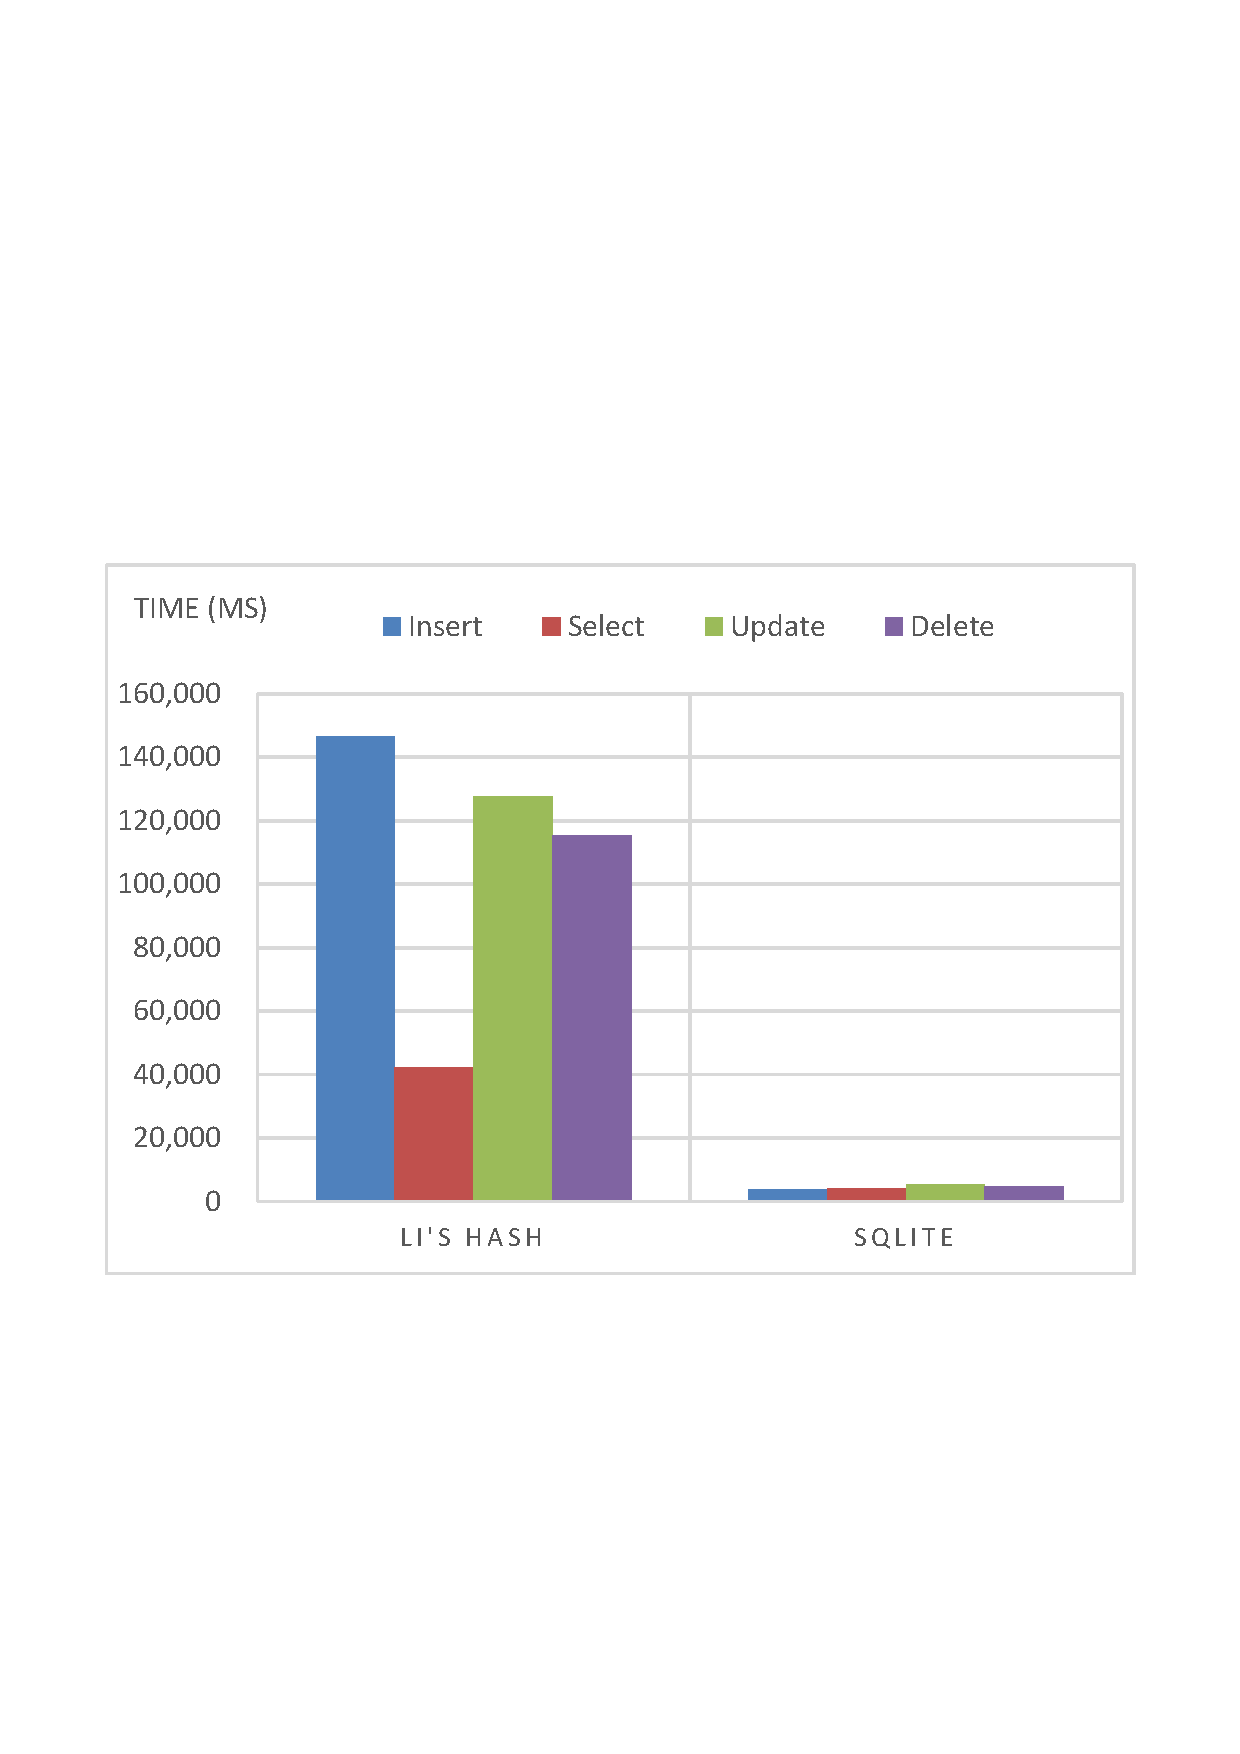
\includegraphics[width=\textwidth]{./performance/result/index-layer/image/100only/real1.pdf}
                \caption{REAL type}
                \label{fig:performance:result:index-layer:insert:string}
        \end{subfigure}

        \caption{Performance on index layer}
        \label{fig:performance:result:index-layer}
\end{figure*}



\clearpage

% ----------------------------------------------------------

% Joining section
\item \textbf{Joining operation}

Joining always is one of the bottleneck of the relational database, but it is just a intersection operation for Li's Hash. So in this test, we let them to do the a mutli-table joining.\\

\begin{figure}[h]
\centering
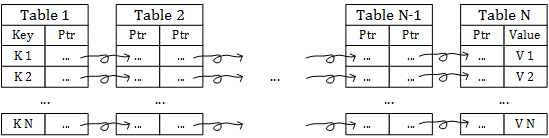
\includegraphics[scale=0.8]{./performance/pic/multi-table_v1.png}
\caption{A example of mutli-table joining.}
\label{fig:performance:multi-table}
\end{figure}

The mutli-table is look like figure \ref{fig:performance:multi-table}, this example is a very sample joining in Human thought, but it still can be a over-hand of the relational database. This example is just search the value by joining many table in the middle, the starting point is the column "Key" in Table 1 and finish is the "Value" column in the Table N, between them is a ton of the pointer which is use for pointing to the next pointer in the next table, so that when search the value which will need to joining these tables and pointer to get the correct value.\\

So this should need to use complex SQL and need times to do that, which will get our a result that the Li's Hash can do the  joining operation and a better time.\\

\clearpage

% ----------------------------------------------------------

\end{enumerate}

% Result section
\subsection{Result}

Figure \ref{fig:performance:result:database-layer} and \ref{fig:performance:result:index-layer} are shows that it is faster after enabled the indexing in SQLite, also Li's Hash become slower because the indexing rather directly using the \textit{put()} or \textit{get()} that because it need to build the index table.\\

In this testing, the main point is not to test how good as the Li's Hash compare to a well-known embedded relational database, but to test it is workable or not, so our will focus on the improvement and the application extension (such as graph database, base on the same table design) to provide different angle and usage.\\

\clearpage

% ------------------------------------------------
% End of page
% ------------------------------------------------
